\par\Needspace{37\baselineskip}\SourceLeaf{272}%
\emph{Gar keine Schwierigkeit hat übrigens die Umformung der Oberfläche eines Revolutionskörpers in die eines andern. Man hat nemlich ($m = \mathit{const.}$):}

\[
\begin{array}{cc}
dy = ds \,.\, \mathit{sin}\varphi & dy' = ds' \,.\, \mathit{sin}\varphi' \\[4pt]
dx = ds \,.\, \mathit{cos}\varphi & dx' = ds' \,.\, \mathit{cos}\varphi'
\end{array}
\]

\[
s = s'
\]

\[
my = y'
\]

\[
m \mathit{sin}\varphi = \mathit{sin}\varphi'
\]

\[
x' = \int dx\, \BareRoot{\left(1 + (1 - mm)\frac{dy^2}{dx^2}\right)}.
\]

\begin{center}\begin{minipage}{\linewidth}\centering
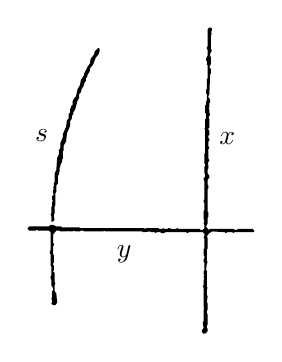
\begin{tikzpicture}[x=0.01039755cm,y=-0.01039755cm]
\fill[even odd rule] (109,42) -- (108,42) -- (104,46) -- (103,50) -- (99,55) -- (98,61) -- (95,65) -- (91,73) -- (91,75) -- (87,81) -- (86,87) -- (83,92) -- (81,101) -- (79,103) -- (77,107) -- (77,111) -- (75,113) -- (75,115) -- (74,116) -- (74,120) -- (72,123) -- (72,128) -- (70,130) -- (69,138) -- (65,147) -- (65,151) -- (62,158) -- (62,164) -- (60,167) -- (60,172) -- (58,176) -- (57,191) -- (55,195) -- (55,206) -- (54,207) -- (54,211) -- (53,212) -- (54,214) -- (53,216) -- (53,219) -- (54,221) -- (52,223) -- (52,227) -- (53,229) -- (52,230) -- (52,235) -- (51,236) -- (51,244) -- (50,245) -- (51,247) -- (51,254) -- (53,254) -- (55,251) -- (54,249) -- (54,245) -- (55,244) -- (55,235) -- (56,234) -- (56,219) -- (57,218) -- (57,210) -- (59,207) -- (59,198) -- (60,197) -- (60,194) -- (61,193) -- (61,188) -- (62,187) -- (62,185) -- (64,181) -- (64,178) -- (65,177) -- (65,168) -- (66,167) -- (66,161) -- (69,156) -- (70,146) -- (74,137) -- (74,131) -- (76,128) -- (76,125) -- (78,122) -- (78,120) -- (80,117) -- (83,106) -- (85,103) -- (85,98) -- (87,96) -- (88,92) -- (91,87) -- (91,85) -- (93,82) -- (93,79) -- (95,77) -- (95,75) -- (98,70) -- (98,67) -- (102,62) -- (105,54) -- (109,49) -- (109,47) -- (110,46) -- (110,43) -- cycle
(246,17) -- (244,17) -- (242,19) -- (242,40) -- (241,41) -- (241,43) -- (242,44) -- (242,51) -- (240,55) -- (240,57) -- (241,58) -- (241,62) -- (242,63) -- (242,79) -- (241,80) -- (241,92) -- (240,93) -- (240,97) -- (241,98) -- (241,106) -- (240,107) -- (240,111) -- (239,112) -- (239,121) -- (240,122) -- (240,128) -- (239,129) -- (239,139) -- (238,140) -- (239,142) -- (239,170) -- (238,171) -- (238,183) -- (239,184) -- (239,186) -- (238,187) -- (238,195) -- (239,196) -- (239,199) -- (237,201) -- (237,203) -- (238,204) -- (238,227) -- (237,228) -- (237,230) -- (238,231) -- (238,240) -- (237,241) -- (237,251) -- (238,252) -- (237,257) -- (238,258) -- (238,262) -- (236,264) -- (233,264) -- (232,263) -- (206,263) -- (205,262) -- (203,263) -- (197,263) -- (196,262) -- (194,262) -- (193,263) -- (189,263) -- (188,262) -- (186,263) -- (183,263) -- (182,262) -- (167,262) -- (166,263) -- (164,262) -- (86,262) -- (85,261) -- (64,261) -- (63,260) -- (57,260) -- (53,258) -- (50,258) -- (48,260) -- (24,260) -- (22,262) -- (22,263) -- (24,265) -- (32,265) -- (33,264) -- (35,265) -- (48,265) -- (50,267) -- (50,289) -- (49,290) -- (49,293) -- (50,294) -- (50,308) -- (51,309) -- (51,320) -- (50,321) -- (50,324) -- (51,325) -- (51,332) -- (53,335) -- (53,338) -- (52,339) -- (52,347) -- (51,348) -- (52,352) -- (51,354) -- (53,356) -- (56,356) -- (58,353) -- (57,342) -- (55,339) -- (55,331) -- (56,330) -- (55,328) -- (55,317) -- (53,315) -- (54,313) -- (54,308) -- (53,307) -- (53,305) -- (54,304) -- (54,295) -- (53,294) -- (53,284) -- (54,283) -- (54,281) -- (53,280) -- (53,270) -- (57,265) -- (61,265) -- (62,266) -- (70,266) -- (71,265) -- (72,266) -- (77,266) -- (78,265) -- (80,266) -- (86,266) -- (87,265) -- (90,265) -- (91,266) -- (114,266) -- (116,265) -- (117,266) -- (162,266) -- (163,267) -- (172,266) -- (173,267) -- (177,267) -- (178,268) -- (180,267) -- (184,267) -- (185,268) -- (189,268) -- (190,267) -- (216,267) -- (217,268) -- (219,267) -- (236,267) -- (238,269) -- (238,272) -- (237,273) -- (238,275) -- (238,287) -- (237,288) -- (237,295) -- (238,296) -- (238,299) -- (237,300) -- (237,303) -- (238,304) -- (238,314) -- (237,315) -- (237,318) -- (238,320) -- (237,322) -- (238,324) -- (237,325) -- (237,332) -- (236,333) -- (237,335) -- (237,358) -- (238,360) -- (237,361) -- (237,376) -- (236,377) -- (237,384) -- (235,387) -- (235,389) -- (237,391) -- (239,391) -- (242,388) -- (242,385) -- (241,384) -- (241,381) -- (242,380) -- (242,367) -- (241,366) -- (241,363) -- (242,362) -- (242,354) -- (241,353) -- (242,345) -- (241,344) -- (241,337) -- (242,335) -- (241,334) -- (241,314) -- (240,313) -- (241,305) -- (242,304) -- (241,302) -- (241,288) -- (242,287) -- (242,274) -- (241,272) -- (244,268) -- (248,266) -- (263,267) -- (264,268) -- (266,267) -- (272,267) -- (273,268) -- (275,267) -- (298,267) -- (299,266) -- (299,265) -- (297,263) -- (279,263) -- (278,264) -- (275,264) -- (274,263) -- (245,263) -- (243,264) -- (240,260) -- (242,256) -- (242,249) -- (243,248) -- (243,243) -- (242,242) -- (242,214) -- (243,213) -- (243,210) -- (242,209) -- (242,203) -- (244,200) -- (244,198) -- (242,195) -- (242,190) -- (243,189) -- (243,185) -- (242,183) -- (244,179) -- (243,177) -- (243,165) -- (244,164) -- (243,162) -- (243,156) -- (244,155) -- (244,153) -- (243,152) -- (243,149) -- (244,148) -- (244,143) -- (243,142) -- (243,140) -- (244,139) -- (244,129) -- (243,127) -- (245,123) -- (244,121) -- (244,117) -- (243,116) -- (244,114) -- (244,109) -- (245,108) -- (245,105) -- (243,102) -- (243,100) -- (244,99) -- (245,74) -- (246,73) -- (246,68) -- (244,65) -- (246,61) -- (246,53) -- (245,52) -- (245,49) -- (247,45) -- (246,43) -- (246,26) -- (247,25) -- (246,22) -- (247,21) -- (247,18) -- cycle;
\node[inner sep=0pt,font=\fontsize{10}{12}\selectfont] at (39,149) {$s$};
\node[inner sep=0pt,font=\fontsize{10}{12}\selectfont] at (266,152) {$x$};
\node[inner sep=0pt,font=\fontsize{10}{12}\selectfont] at (140,294) {$y$};
\end{tikzpicture}

\end{minipage}\end{center}

\emph{Für die Curve, durch deren Revolution das Gegenstück der Kugel entsteht, ist:}

\[
y = R \mathit{sin}\varphi
\]

\[
x = R \mathit{cos}\varphi + \mathit{log} \mathit{tang}\, \tfrac{1}{2}\varphi
\]

\[
s = R \mathit{log} \frac{1}{\mathit{sin}\varphi}.
\]

\begin{center}\begin{minipage}{\linewidth}\centering
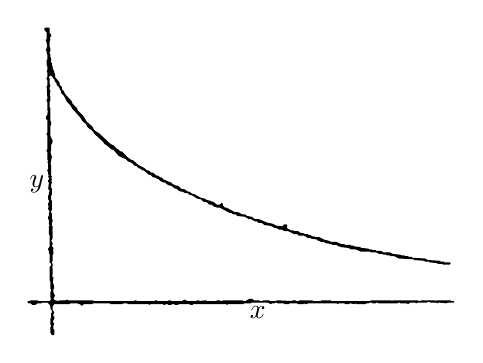
\begin{tikzpicture}[x=0.00965058cm,y=-0.00965058cm]
\fill[even odd rule] (32,15) -- (32,17) -- (35,20) -- (35,29) -- (34,30) -- (34,32) -- (35,33) -- (35,36) -- (36,37) -- (34,44) -- (35,45) -- (35,48) -- (36,49) -- (36,56) -- (35,57) -- (35,64) -- (36,65) -- (36,70) -- (35,71) -- (36,73) -- (36,79) -- (35,80) -- (35,82) -- (36,83) -- (36,90) -- (35,91) -- (36,108) -- (35,109) -- (35,111) -- (36,112) -- (36,123) -- (37,125) -- (36,126) -- (36,129) -- (34,131) -- (34,134) -- (36,136) -- (36,152) -- (35,153) -- (35,155) -- (36,156) -- (36,174) -- (35,175) -- (35,177) -- (36,178) -- (36,188) -- (37,189) -- (36,191) -- (37,193) -- (37,200) -- (36,201) -- (36,203) -- (37,204) -- (37,207) -- (38,208) -- (37,210) -- (38,212) -- (38,214) -- (37,215) -- (37,217) -- (38,218) -- (37,226) -- (39,229) -- (38,231) -- (38,234) -- (37,235) -- (37,240) -- (38,241) -- (38,244) -- (37,245) -- (37,248) -- (38,250) -- (37,251) -- (37,253) -- (39,256) -- (38,258) -- (38,262) -- (37,263) -- (37,266) -- (38,267) -- (38,273) -- (39,274) -- (38,276) -- (38,286) -- (39,287) -- (39,302) -- (37,305) -- (37,307) -- (38,308) -- (38,311) -- (39,312) -- (39,323) -- (41,325) -- (41,327) -- (39,329) -- (39,347) -- (40,348) -- (40,358) -- (41,359) -- (41,361) -- (40,362) -- (40,370) -- (41,372) -- (39,374) -- (24,374) -- (23,373) -- (14,373) -- (13,374) -- (10,374) -- (10,376) -- (11,377) -- (14,377) -- (16,379) -- (20,379) -- (23,377) -- (28,377) -- (29,376) -- (36,376) -- (39,379) -- (40,381) -- (40,384) -- (42,387) -- (42,389) -- (41,390) -- (41,396) -- (40,397) -- (40,405) -- (41,406) -- (40,408) -- (40,416) -- (42,419) -- (44,419) -- (45,418) -- (45,412) -- (44,411) -- (44,406) -- (45,404) -- (43,401) -- (45,397) -- (45,395) -- (44,394) -- (44,391) -- (45,389) -- (43,386) -- (43,381) -- (45,378) -- (65,378) -- (66,377) -- (76,377) -- (77,378) -- (79,378) -- (81,380) -- (82,380) -- (84,378) -- (95,378) -- (96,377) -- (118,377) -- (119,378) -- (135,378) -- (136,377) -- (141,377) -- (142,378) -- (169,378) -- (170,379) -- (172,378) -- (188,378) -- (189,379) -- (191,379) -- (192,378) -- (194,378) -- (195,379) -- (199,379) -- (200,378) -- (203,378) -- (204,379) -- (208,379) -- (209,378) -- (223,378) -- (224,379) -- (227,379) -- (228,378) -- (271,378) -- (273,379) -- (274,378) -- (294,378) -- (295,377) -- (304,377) -- (305,376) -- (326,376) -- (330,378) -- (332,377) -- (335,377) -- (336,376) -- (338,376) -- (339,377) -- (347,377) -- (348,378) -- (354,378) -- (355,377) -- (365,377) -- (366,378) -- (373,378) -- (374,377) -- (376,378) -- (378,378) -- (379,377) -- (417,377) -- (418,378) -- (420,377) -- (427,377) -- (428,378) -- (433,378) -- (434,377) -- (440,378) -- (442,377) -- (443,378) -- (455,378) -- (456,377) -- (459,377) -- (460,376) -- (463,376) -- (464,377) -- (468,377) -- (469,376) -- (471,376) -- (472,377) -- (497,377) -- (498,376) -- (500,376) -- (501,377) -- (509,377) -- (511,378) -- (514,376) -- (520,376) -- (522,377) -- (523,376) -- (536,376) -- (537,375) -- (539,375) -- (540,376) -- (548,376) -- (549,377) -- (551,376) -- (562,377) -- (563,376) -- (571,376) -- (572,375) -- (571,374) -- (568,374) -- (567,373) -- (549,373) -- (548,374) -- (546,373) -- (528,373) -- (527,374) -- (525,374) -- (524,373) -- (491,373) -- (490,374) -- (488,373) -- (462,373) -- (461,374) -- (410,374) -- (409,373) -- (397,373) -- (396,374) -- (386,374) -- (385,373) -- (368,373) -- (367,374) -- (364,374) -- (363,373) -- (359,373) -- (358,374) -- (338,373) -- (337,374) -- (329,374) -- (328,373) -- (320,373) -- (319,374) -- (316,374) -- (315,373) -- (308,373) -- (306,371) -- (302,371) -- (297,374) -- (294,374) -- (293,373) -- (267,373) -- (266,374) -- (264,374) -- (263,373) -- (259,373) -- (258,374) -- (246,374) -- (245,373) -- (236,374) -- (235,373) -- (233,373) -- (232,374) -- (220,374) -- (217,372) -- (213,374) -- (199,374) -- (198,373) -- (196,373) -- (195,374) -- (181,374) -- (180,373) -- (178,373) -- (177,374) -- (154,374) -- (153,373) -- (151,373) -- (150,374) -- (97,374) -- (96,373) -- (63,373) -- (62,372) -- (60,373) -- (52,373) -- (51,374) -- (46,373) -- (44,371) -- (46,367) -- (44,363) -- (44,358) -- (45,357) -- (44,351) -- (43,350) -- (44,343) -- (42,341) -- (43,339) -- (43,331) -- (42,330) -- (43,328) -- (43,325) -- (42,324) -- (42,322) -- (43,321) -- (43,313) -- (44,312) -- (44,309) -- (43,307) -- (44,306) -- (44,304) -- (42,302) -- (43,298) -- (41,295) -- (43,291) -- (43,282) -- (42,281) -- (43,279) -- (43,276) -- (42,275) -- (42,270) -- (43,269) -- (43,267) -- (42,266) -- (42,259) -- (41,258) -- (41,255) -- (42,254) -- (42,242) -- (41,241) -- (41,235) -- (42,234) -- (42,226) -- (41,225) -- (41,220) -- (42,218) -- (41,216) -- (42,214) -- (41,212) -- (42,210) -- (41,209) -- (41,195) -- (40,194) -- (42,183) -- (41,182) -- (40,177) -- (41,176) -- (41,168) -- (42,167) -- (43,163) -- (40,157) -- (40,143) -- (41,142) -- (41,138) -- (40,137) -- (40,120) -- (39,119) -- (39,111) -- (40,110) -- (40,104) -- (39,103) -- (40,97) -- (39,96) -- (39,92) -- (40,90) -- (39,89) -- (39,81) -- (38,80) -- (38,79) -- (40,77) -- (41,77) -- (45,82) -- (46,85) -- (48,87) -- (48,89) -- (51,92) -- (54,98) -- (54,100) -- (58,104) -- (62,112) -- (66,116) -- (69,121) -- (79,132) -- (82,137) -- (87,141) -- (88,144) -- (92,148) -- (93,148) -- (97,152) -- (97,153) -- (110,165) -- (110,166) -- (112,168) -- (113,168) -- (120,174) -- (123,175) -- (130,183) -- (139,187) -- (142,190) -- (147,192) -- (151,196) -- (153,196) -- (156,199) -- (159,200) -- (161,202) -- (163,202) -- (170,208) -- (172,208) -- (175,211) -- (177,211) -- (183,214) -- (185,216) -- (189,218) -- (191,218) -- (193,220) -- (197,222) -- (199,222) -- (204,226) -- (206,226) -- (208,228) -- (212,230) -- (214,230) -- (218,232) -- (221,232) -- (223,234) -- (227,235) -- (233,239) -- (238,240) -- (241,243) -- (246,244) -- (249,247) -- (252,247) -- (256,250) -- (258,250) -- (259,251) -- (263,251) -- (276,258) -- (278,258) -- (281,260) -- (284,260) -- (286,262) -- (296,263) -- (301,266) -- (304,266) -- (309,269) -- (312,269) -- (314,271) -- (318,271) -- (322,274) -- (330,275) -- (336,278) -- (338,278) -- (341,280) -- (345,280) -- (348,282) -- (353,282) -- (361,286) -- (365,286) -- (367,288) -- (374,288) -- (379,291) -- (383,291) -- (384,292) -- (391,293) -- (393,295) -- (395,295) -- (396,296) -- (400,296) -- (403,298) -- (406,298) -- (407,299) -- (410,299) -- (411,300) -- (417,300) -- (419,302) -- (421,302) -- (422,303) -- (432,304) -- (436,306) -- (442,306) -- (449,309) -- (461,309) -- (462,310) -- (469,310) -- (473,312) -- (477,312) -- (478,313) -- (482,313) -- (483,314) -- (487,314) -- (488,315) -- (493,315) -- (499,318) -- (518,319) -- (519,320) -- (532,321) -- (533,322) -- (538,322) -- (539,323) -- (549,324) -- (550,325) -- (556,325) -- (557,326) -- (566,326) -- (567,324) -- (566,323) -- (559,323) -- (558,322) -- (554,322) -- (553,321) -- (537,320) -- (533,318) -- (517,317) -- (516,316) -- (512,316) -- (511,315) -- (507,315) -- (506,314) -- (502,314) -- (501,313) -- (491,312) -- (487,310) -- (479,310) -- (475,308) -- (469,308) -- (468,307) -- (464,307) -- (463,306) -- (460,306) -- (459,305) -- (449,304) -- (448,303) -- (440,302) -- (439,301) -- (436,301) -- (435,300) -- (428,300) -- (427,299) -- (423,299) -- (416,296) -- (409,296) -- (408,295) -- (400,293) -- (394,290) -- (389,290) -- (388,289) -- (385,289) -- (382,287) -- (380,287) -- (379,286) -- (375,286) -- (374,285) -- (369,284) -- (366,282) -- (361,282) -- (360,281) -- (357,281) -- (353,279) -- (351,277) -- (352,275) -- (351,273) -- (348,273) -- (345,276) -- (343,275) -- (338,275) -- (332,272) -- (326,271) -- (314,266) -- (309,266) -- (305,263) -- (299,262) -- (296,260) -- (293,260) -- (287,257) -- (283,257) -- (272,251) -- (270,251) -- (267,248) -- (267,246) -- (266,245) -- (265,245) -- (263,247) -- (259,247) -- (254,243) -- (252,243) -- (251,242) -- (246,241) -- (243,239) -- (238,238) -- (229,233) -- (227,233) -- (223,230) -- (221,230) -- (217,227) -- (212,226) -- (208,222) -- (205,222) -- (201,220) -- (199,218) -- (189,214) -- (186,211) -- (184,211) -- (182,209) -- (180,209) -- (175,205) -- (173,205) -- (169,202) -- (167,202) -- (164,199) -- (156,195) -- (148,188) -- (146,188) -- (144,186) -- (143,186) -- (134,177) -- (132,177) -- (129,174) -- (128,174) -- (123,169) -- (119,167) -- (104,153) -- (99,150) -- (97,148) -- (95,144) -- (88,138) -- (83,130) -- (76,123) -- (75,120) -- (69,114) -- (68,111) -- (59,101) -- (58,98) -- (55,95) -- (55,92) -- (52,89) -- (52,86) -- (46,79) -- (46,75) -- (45,74) -- (45,72) -- (43,68) -- (43,65) -- (42,64) -- (42,61) -- (41,60) -- (41,54) -- (40,53) -- (40,49) -- (39,48) -- (39,46) -- (40,45) -- (40,41) -- (39,40) -- (39,32) -- (40,30) -- (39,28) -- (41,25) -- (41,23) -- (39,21) -- (39,15) -- (38,14) -- (33,14) -- cycle;
\node[inner sep=0pt,font=\fontsize{10}{12}\selectfont] at (22,220) {$y$};
\node[inner sep=0pt,font=\fontsize{10}{12}\selectfont] at (313,389) {$x$};
\end{tikzpicture}

\end{minipage}\end{center}

\begin{center}
\begin{tabular}{c|c|c|c}
$\varphi$ & $y$ & $x$ & $s$ \\
\hline
$0^0$ & 0.0000 & $\infty$ & $\infty$ \\
$10^0$ & 0.1736 & 1.45144 & 1.75072 \\
$20^0$ & 0.3420 & 0.79572 & 1.07289 \\
$30^0$ & 0.5000 & 0.45095 & 0.69315 \\
$40^0$ & 0.6428 & 0.24464 & 0.44194 \\
$50^0$ & 0.7660 & 0.12012 & 0.26652 \\
$60^0$ & 0.8660 & 0.04931 & 0.14384 \\
$70^0$ & 0.9397 & 0.01436 & 0.06220 \\
$80^0$ & 0.9848 & 0.00178 & 0.01531 \\
$90^0$ & 1.0000 & 0.00000 & \\
\end{tabular}
\end{center}

Bei der Tabelle beachte man, dass die Logarithmen natürliche, nicht \textsc{Brigg}ische sind.

\hfill \textsc{Stäckel}.
